\chapter{Library-on-library profiling of protein binding landscapes}


\newthought{Antibodies and antibody like proteins} (binders) are incredibly important therapeutic modalities and research tools \cite{Weiner2015-om}. Together, binders make approximately 98 billion dollars of revenue, with over 60 monoclonal antibodies approved \cite{Singh2018-pk,Ecker2015-jl}. In research, binders enable the functional probing of living systems to determine the mechanisms by which molecules dictate the functions of life. Binders can be used to inhibit, deplete, activate or detect molecules (targets) within a cell, enabling us to infer the importance of the probed molecule\cite{Rhodes2006-za}. Despite these successes, there is still room for improvement; an estimated X\% of binders fail in phase II clinical trials\cite{Ecker2015-jl} and an estimated 800 million dollars are wasted using binders with poor specificity in research\cite{Bradbury2015-hm}. Current screening methods pan a library of binders against a single target, often developing strong affinity, but ignoring contextual function as well as specificity. Furthermore, usually only the top “hits” are tested, not enabling learning of the sequence determinants of binding.  To address these challenges, we develop a method for assaying libraries of binders against libraries of targets at the tera-scale. Importantly, the method uses sequencing as a readout, providing functional characterization of antibodies from both positive and negative data. Using data generated from this method, we build models learn the sequence determinants of binding, and design binders predicted to have not only high affinity but also high specificity to a given target in a competitive context of a cell. This work enables a future of measurement driven antibody design, empowered by machine learning and high-throughput synthesis and sequencing methods.

\section{Binder utility and discovery} 

Over the past five decades, binders have transformed the therapeutic and research landscape by virtue of their ability to inhibit and detect other molecules of interest\cite{Kohler1975-oz}. Since the development of the methods for generating specific monoclonal antibodies\cite{Kohler1975-oz,Rossant2014-cf}, we have used binders to detect the presence of the protein they bind to (target) via methods such as the western blot and ELISA\cite{Engvall1971-ff,Burnette1981-nc}. Binders can further be used more in line with the physiological function to neutralize a target of interest in vivo, a method we have co-opted for use in therapeutics. This form of medicine has transformed the way he treat patients and opened up a class of targets not thought possible to target with small molecules. Taken together, binding has been one of the most important tools of biology this century. 

While their has been great progress in binder engineering and development, many challenges remain\cite{Schonbrunn2014-nb,Parseghian2013-rq,Rhodes2006-za,Herrera2013-wm,Mechetner2011-cm,Perkel2014-df,Weller2016-xv}. A meta study which aimed to reproduce 63 different studies of interest found that only X\% were able to be reproduced\cite{Begley2012-vv}. Furthermore, approximately 72\% of clinical trials for binders fail in phase 2\cite{Ecker2015-jl}. A recent study which developed methods to probe the specificity of binders using mass spec found high variation in specificity of binders to a given target, even when purchased from the same provider\cite{Marcon2015-qr}. When developing binders for use in therapeutics, there are biophysical properties of interest which are often neglected and ignored when developing antibodies\cite{Jain2017-zg}, likely leading to higher rates of variability in research and clinical failures. Many of the challenges arise from the methods we use to engineer binders, which have not changed much in the preceding 30 years. 

Our ability to engineer binders which hit specific target proteins of interest has lead to thousands of binders being available to many targets across protein domains domains. Engineering initially---and often still---is done via hybridoma methods\cite{Kohler1975-oz}, where an animal is injected with a target of interest and the resulting B-cells which produce antibodies are purified and tested for target binding. This approach is time consuming and costly. Phage display was developed as a way to rapidly screen more than millions of possible sequences against a target of interest very rapidly and for low cost\cite{Hoet2005-qp}. While fast and cheap, phage display does not always succeed in delivering antibodies with quality chemical properties desired,  such as folding and stability\cite{Jain2017-zg}. This further lead to yeast display, using a similar method except on the surface of yeast, further “humanizing” the abinders displayed and enriching their chance of being successful in therapeutic concepts\cite{Boder1997-gx,Boder2000-ej}. While these methods screen millions of binders at once, they generally are limited on the target side to screening an individual target. The more recent development of these in vitro methods to screen antibodies has enabled the screening of synthetic binding designs, further the type of properties one can develop into a binder. 

While antibodies currently remain the main therapeutic modality, synthetic binders enable properties outside the scope of antibodies to be developed, furthering different goals in research and therapeutics\cite{Yu2017-qj}. Antibodies function incredibly well in the blood, however their ability to penetrate barriers---such as the blood brain--- are limiting\cite{Thom2018-ka}. Antibodies also contain many disulfide bonds, limiting their ability to function inside a cell\cite{Edelman1961-eg,Lo2008-qq}. This also makes them challenging to produce in a simpler organism such as E coli, and therefore expensive to produce. While antibodies have long half lives, this can also be detrimental in certain research and therapeutic situations, such as when the effect of a drug is toxic.

Synthetic binders aim to address some of these challenges. There are many types of synthetic binders\cite{Yu2017-qj,Murali2012-tq,Krehenbrink2008-aj,Behar2013-ya,Desmet2014-ir,Richter2014-ll,Parmeggiani2008-tf,Boersma2011-kc,Schlatter2012-ay,Duan2007-hs,Binz2005-st,Nygren2008-tj,Vazquez-Lombardi2015-se}, which access many different structural motifs useful for binding diverse targets. Many of these scaffolds are smaller and simpler than antibodies, allowing them to be synthesized in bacteria. Scaffold diversity abounds across many different constructs; fibronectin domains (adnectins) are based on human proteins and have structures similar to immunoglobulins\cite{Dineen2008-im}, while alphabodies are entirely synthetically constructed helices with variable positions displayed throughout the helix\cite{Desmet2014-ir}. The diversity of structures can be useful when attempting to make binders against hard targets, however synthetic binders contain challenges of their own. 

Synthetic binders have remained lagging behind mAbs in their ability to be developed as therapeutics. Therapeutically, they are often degraded in the human context quite quickly. Immune responses remain an unsolved challenge as well. The more synthetic a construct is, the more likely an animal is to raise an immune response towards it, thus neutralizing any future introduction of the binder. Furthermore, synthetic constructs can be plagued by similar challenges in terms of production and developability, often not folding correctly and struggling to be produced. 

A major challenge across any binder scaffold and development method is specificity\cite{Schonbrunn2014-nb,Parseghian2013-rq,Rhodes2006-za,Herrera2013-wm,Mechetner2011-cm,Perkel2014-df,Weller2016-xv}. Since binders are often screened against a single target at one time, no information is gleaned in regards to how that bidner will function in the competitive environment of a cell or animal. Furthermore, usually individual hits are tested, thus no information is learned in regards to the distribution of binding properties across the entire library. However, exciting developments in next-gen synthesis and sequencing, in combination with machine learning, provide a path towards more targeted design of binder modalities. 

 Recently, an explosion in high-throughput measurement methods, as well as protein modeling methods have lead to exponential leaps in our understanding and abilities to design proteins. Working using the software Rosetta\cite{Chevalier2017-zf} has highlighted the ability to make functional structures based on de novo protein modeling.  Furthermore, leveraging methods of DNA chip synthesis has enabled the construction of thousands of sequences which can then be probed for function across relevant environments\cite{Melnikov2012-oc,Starita2015-uk}. There have also been exciting developments in high-throughput assays; 2 hybrids measuring interactions of proteins have been adapted to allow for library-on-library measurement, in a method which typically held one side of the reaction constant\cite{Yachie2016-ss,Trigg2017-hz,Younger2017-as}. 

An ideal method for screening binders would allow for many binders to be screened against many targets, in a way that is easily readable using sequencing, and amenable to machine learning methods and future rounds of design. To this end, we have developed a highly parallel method which facilitates the measurement of millions of binders against millions of targets in a single reaction. The interactions are measured via simple NGS of short barcodes. Using this method, we apply machine learning approaches to learn the structure of our data, in an effort to learn the code of how binders and targets interact. 

\section{Results}
\subsection{Development of a library on library high throughput screening method}

%Figure 1: Library design
\begin{figure}[b!]
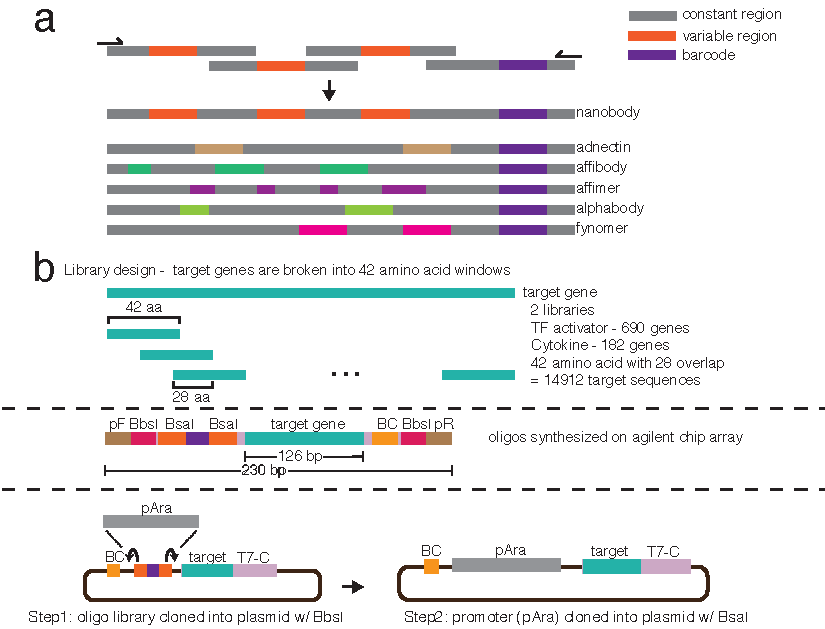
\includegraphics[width=\textwidth]{figures/chapter3/20190621_fig1_design_and_t7.pdf}
\caption[Construction of binder and target libraries for assaying interactions]{\textbf{Construction of binder and target libraries for assaying interactions.}
a, Binders are synthesized in 200 base pair partitions, and assembled using PCR. Barcodes are added to the 3 prime sequence end. b, Target genes are broken into 42 amino acid fragments, and a sliding window is scanned along the gene so fragments overlap. This fragment is synthesized using chip based methods, and cloned into a plasmid using a 2 step process to generate the full length library construct.
\label{chap3-library-design}}
\end{figure}

First we synthesized binder and target libraries across a diverse array of proteins and scaffolds. We constructed 5 binder libraries based on previously developed scaffolds: adnectins, affibody, affimers, fynomers, and nanobodies (Fig\ref{chap3-library-design}a). Each library was constructed using DNA synthesis with controlled codon randomization allowing for all amino acids to be represented without stop codons (Methods). These synthesized oligos (ranging from 2-5 total oliogs of 200bp length) were then assembled through overlap extension PCR\cite{Urban1997-ri}, adding a barcode to the gene 3 prime tail, and cloned into a plasmid construct. 

Target libraries were synthesized using Agilent chip synthesis (Fig\ref{chap3-library-design}b). All human cytokines (186 total genes) and ~75\% of human transcription factor activators were chosen to be the initial target libraries, blanketing diversity across different protein functional classes. Each gene was synthesized in 42 amino acid windows, which overlapped by 28 amino acids. This accounted for 14912 unique target sequences representing these genes. Each target sequence was barcoded during synthesis, and then cloned into plasmid connecting it to the downstream c-term of split T7. This approach of scanning small slices of full target genes enables direct mapping of binders to specific regions of proteins, an important consideration for downstream machine learning. Both of these libraries were put through our recombination pipeline to create dually barcoded plasmid ORFs. 

In order to measure billions of interactions across a library on library space, we developed a plasmid recombination system in E coli that scales linearly with culture size (Fig\ref{chap3-recombine-T7}a). The epitope library contains an F1 origin, allowing for packaging of the plasmid inside phage. After cloning, a plasmid containing helper phage genes was electroporated into the e coli with the target library, which starts the process of phage production. Phage containing the epitope plasmids were then purified (methods). The binder library was cloned into a strain harboring the F plasmid, as well as a reporter plasmid containing BxbI recombinase under Lac inducible expression, and a T7 promoter controlling Kan-SSRA and GFP. These cells were then infected by phage, and recombination was induced for 4 hours. After 4 hours, selection for all plasmid was added, and cells were either back diluted, or plated on plates containing all selection markers for calculation of recombination efficiency. Recombination efficiency is estimated to be approx 10\% of total cells on average across many replicates (Fig\ref{chap3-recombine-T7}a), a phenomenon which scales linearly with culture volumes. Recombination was carried out for each binder and target pairing individually, to not allow for any one library to take over the pool. This method enables incredibly large scale interaction libraries to be created (approximately 1e11 per liter of e coli culture). 

%Figure 2: Phage assisted recombination enables measurement of billions of interactions
\begin{figure}[t]
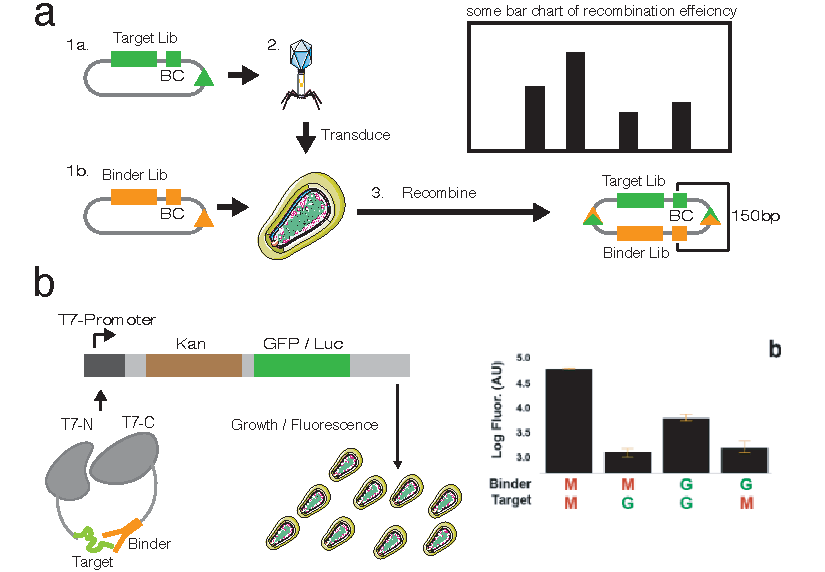
\includegraphics[width=\textwidth]{figures/chapter3/20190621_fig2_recombine_and_t7.pdf}
\caption[Phage assisted recombination enables measurement of billions of interactions]{\textbf{Phage assisted recombination enables measurement of billions of interactions.}
a, Target library is cloned and packaged in phage. Phage transduces and delivers library into cells containing the binder library, as well as a vector which induces recombination of the two plasmids.  b, Split T7 assay for testing interaction. If a binder-target pair interacts, transcription is activated at a T7 promoter, inducing Kan and GFP expression.
\label{chap3-recombine-T7}}
\end{figure}

In order to screen interactions at scale. A split T7 system was leveraged\cite{Pu2017-zo} to drive the T7 promoter on the reporter plasmid. Target libraries were connected to the T7 N-terminus, while binder libraries were connected to the C-terminus. If a binder target pair interact, this drives transcription from the T7 promoter, selecting for these cells upon outgrowth (Fig\ref{chap3-recombine-T7}b). These cells can be further screened via flow cytometry or cell sorting for fluorescence, also driven by the T7 promoter. This split T7 system was tested using control nanobodies binding to two distinct targets, mCherry and GFP, and shown to provide high signal to background ratios (Fig\ref{chap3-recombine-T7}b). 

To select for cells which contain interacting pairs, recombined culture was back diluted and expression of the split T7 components was induced for 4 hours (Fig\ref{chap3-lib-assay}a. At induction, a time point was collected (T=0) to estimate the culture diversity. After induction for 2 hours, cells were back diluted 10x and Kanamycin was added to select for interactions. At 2 hours, another time point (T=1) was collected, and the cells were again back diluted 10x. After overnight growth, one final time point was collected (T=2) (Fig 2). Diversity of the samples was assessed via Illumina sequencing of barcodes. 

%Figure 3: Library assay design for measuring billions of binding interactions
\begin{figure}[t]
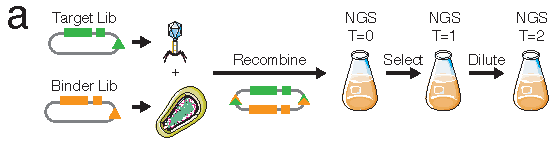
\includegraphics[width=\textwidth]{figures/chapter3/20190621_fig3_selection_description.pdf}
\caption[Library assay for measuring interactions]{\textbf{Library assay for measuring interactions.}
a, Library is recombined, then kanamycin selection is added.The bacteria is back diluted twice and sampled at each timepoint to determine distribution of binder-target pairs via NGS.
\label{chap3-lib-assay}}
\end{figure}

%Experimental Results of binder-target library on library assay
Timepoints were initially assessed to analyze library diversity. Diversity can either be considered from three perspectives: the binder, the target, for the binder target pairing. Across all the libraries, diverse distributions for the individual library components were observed. In the T=0 timepoints, target (Fig\ref{chap3-target-histograms}a) library distributions were observed to be approximately log normal distributed (Fig\ref{chap3-target-histograms}b). This is as expected, considering these libraries are quite small in comparison to total recombined library size, and they have yet to undergo selection. As the time points progressed, the target library distribution was bottlenecked, showing certain sequences were lost and others were enriched (Fig\ref{chap3-target-histograms}c). This likely indicates selection for specific binding interactions, and other sequences not being bound or having fitness defects. 

%Figure 4: Target barcode distribution across measurements
\begin{figure}
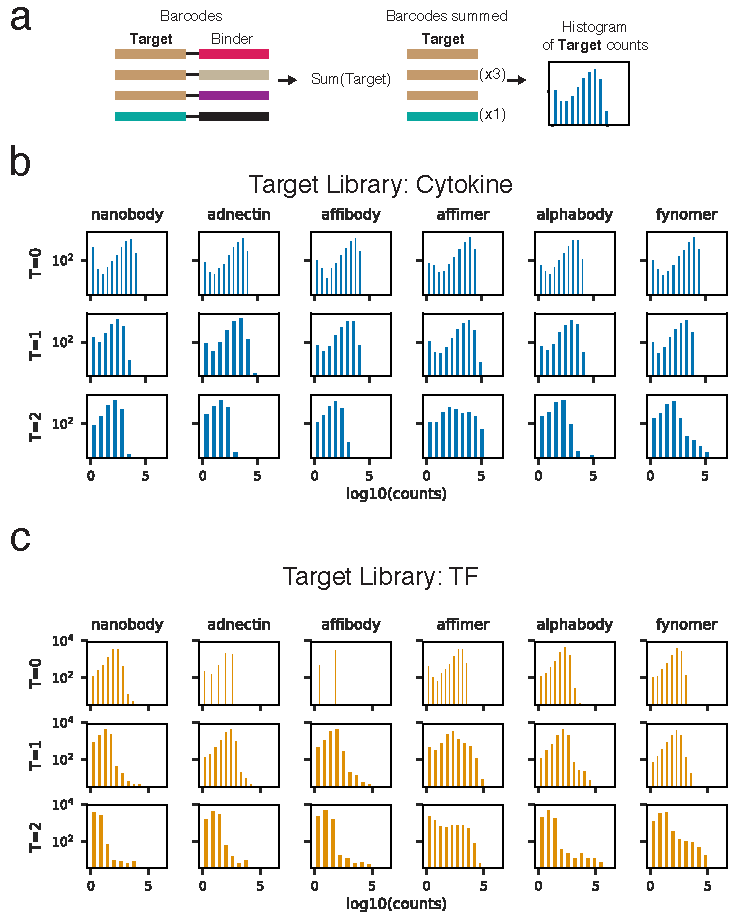
\includegraphics[width=\textwidth]{figures/chapter3/20190621_fig4_target_histograms.pdf}
\caption[Distribution of targets across timepoints]{\textbf{Distribution of targets across timepoints}
a, after counting barcodes, all counts for a given target are summed, then the distribution is plotted. b, Target distribution for the cytokine target library across the different binder libraries tested. c, Target distribution for the TF target library across the different binder libraries tested.
\label{chap3-target-histograms}}
\end{figure}

%Figure 5: Binder barcode distribution across measurements
\begin{figure}
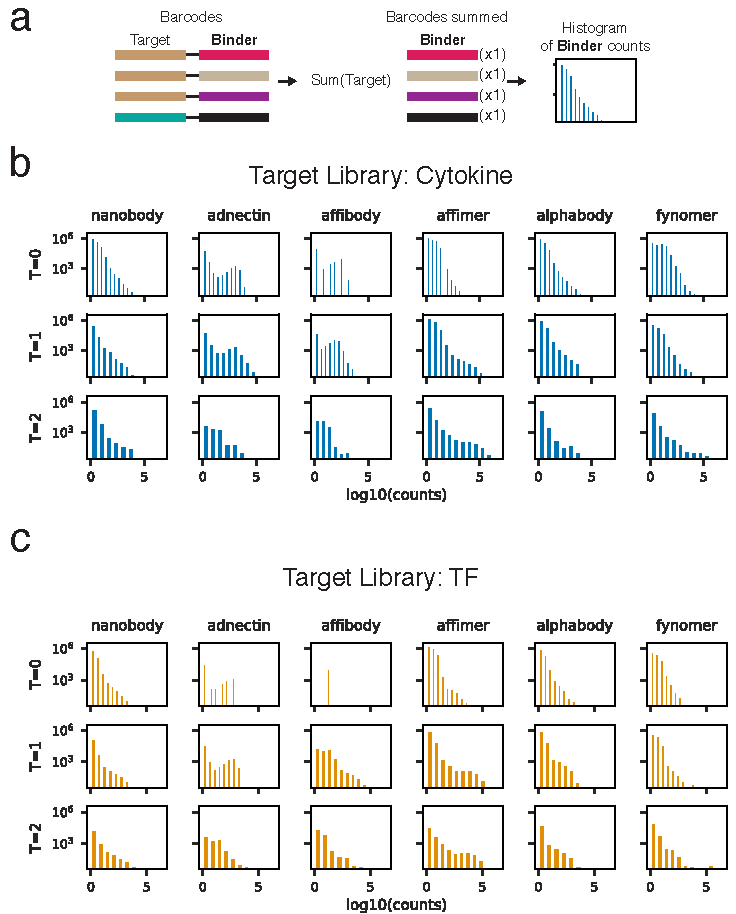
\includegraphics[width=\textwidth]{figures/chapter3/20190621_fig5_binder_histograms.pdf}
\caption[Distribution of binders across timepoints]{\textbf{Distribution of binders across timepoints}
a, after counting barcodes, all counts for a given binders are summed, then the distribution is plotted. b, Binder distribution for the cytokine target library across the different binder libraries tested. c, Binder distribution for the TF target library across the different binder libraries tested.
\label{chap3-binder-histograms}}
\end{figure}

%Figure 6: Selection across libraries
\begin{figure}
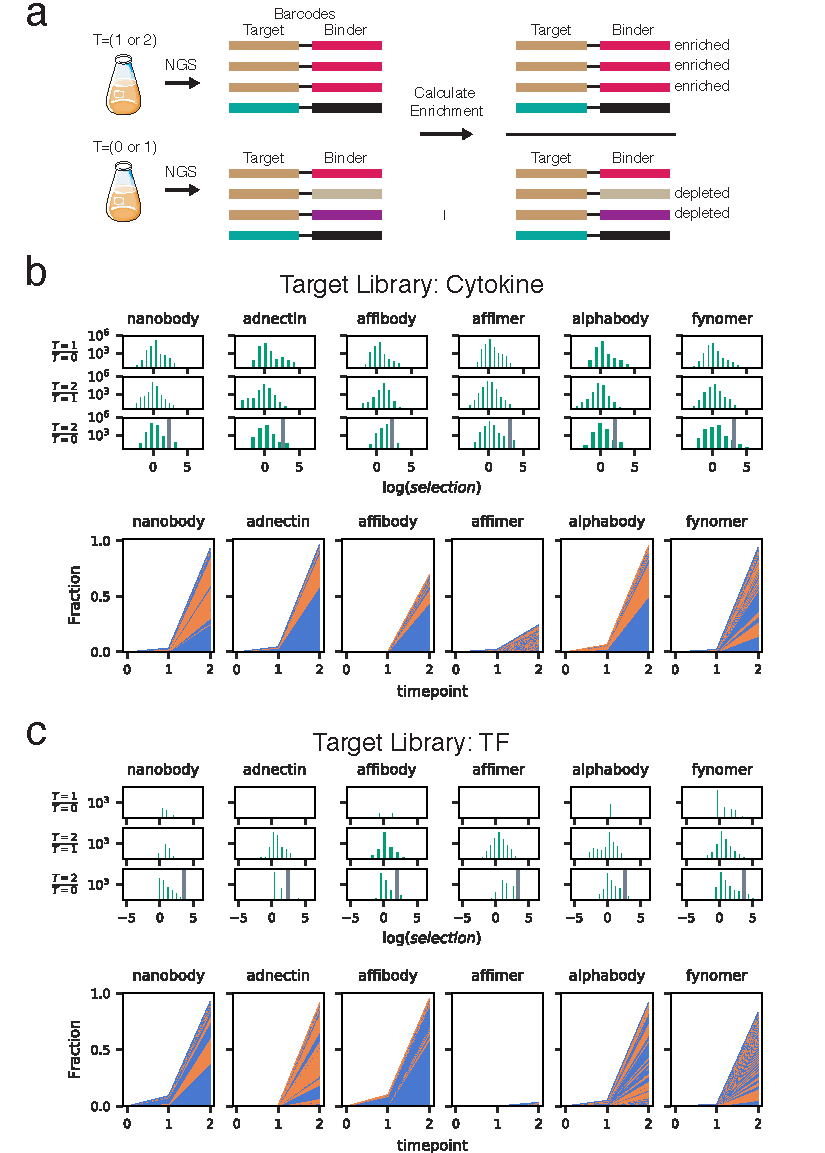
\includegraphics[width=.9\textwidth]{figures/chapter3/20190621_fig6_enrichment_histograms.pdf}
\centering
\caption[Enrichment of binder-target pairs across timepoints]{\textbf{Enrichment of binder-target pairs across timepoints}
\label{chap3-selection-histograms}}
\end{figure}

%Fig 7: Library on library enrichment values across different libraries
\begin{figure}
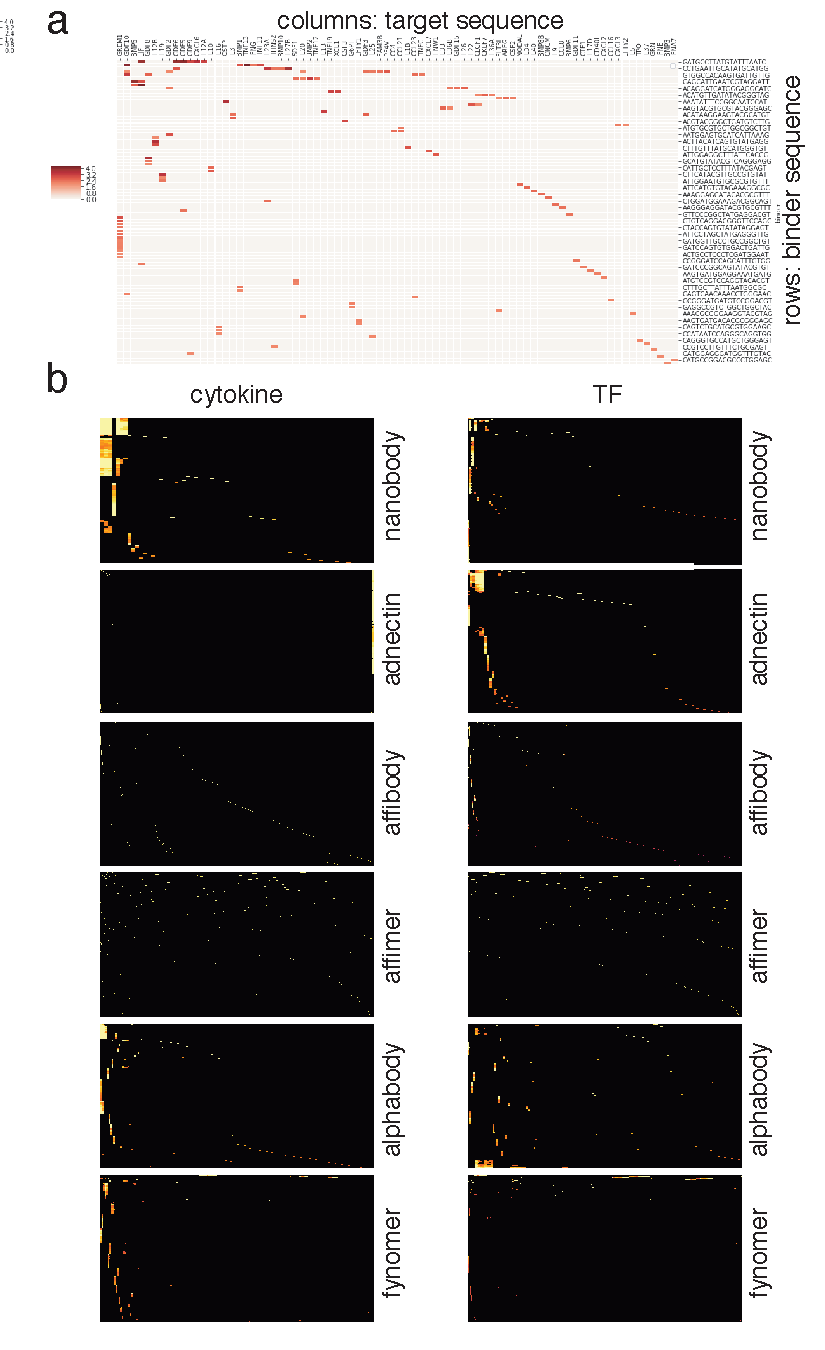
\includegraphics[width=\textwidth]{figures/chapter3/20190621_fig7_selection_clustermaps.pdf}
\caption[Clustering of top binder-target interactions]{\textbf{Clustering of top binder-target interactions}
\label{chap3-selection-clusters}}
\end{figure}

 Across the initial timepoints, binder libraries contained massive diversity, with most sequences only be counted a single time on hundreds of millions of reads (Fig\ref{chap3-binder-histograms}a/b). This too is expected, considering the only bottleneck these libraries were exposed to was cloning transformation. After selection, restricted population of binders across each of the libraries became log normally distributed (Fig\ref{chap3-binder-histograms}a/b). The total population size of each library depended on the binding scaffold used, and varied widely from under 100 sequences to millions (Table 1). This likely is a function of the initial library diversity, but also the binding properties of the scaffolds as well. 

Enrichment values for interacting target protein pairs seen in both time point T=1 and T=2 were calculated. Of note, not all sequences were positively enriched in T=2, and there is negative as well as positive selection (Fig\ref{chap3-selection-histograms}). This could be because certain pairs contain such strong interaction that they drive more growth, or because the initial T=1 time point still contained background needing to be further diluted. These selection values were then parsed for some binder target pairs with the largest enrichment values. Interestingly, there was a diversity of specificity patterns seen from both the binder perspective as well as the target perspective (Fig Figure 6b/c). Certain binders were non-specific and bound tightly to multiple targets, while also some targets (notably GMPxx) bound to many different binder sequences, even across libraries. This finding could only be determined by using a library on library screening method as such. While further validation will be needed to follow up, this points to an interesting consideration when designing binders as well as choosing targets. 

The interactions illustrated in (Fig\ref{chap3-selection-clusters}) represented only XXX fraction of the total data. All in all, ~700 thousand enrichment values were calculated, meaning that many pairs were seen in both T=1 and T=2 across the libraries. Accounting for all data in T=0,T=1, and T=2 timepoints, over 5 million different binder-target pairs were measured. This type of diverse and rich data structure is highly amenable to a machine learning assisted approach, allowing for further functional annotation and directing future rounds of design. 

\subsection{Machine learning guided functional determination}

% Figure 8: MLP model is able to accurately predict across many sequence types. 
\begin{figure}
\includegraphics[width=\textwidth]{figures/chapter3/20190621_fig8_model_analysis.pdf}
\caption[Multi-layer perceptron learns binder-target properties based on sequence determinants]{\textbf{Multi-layer perceptron learns binder-target properties based on sequence determinants}
\label{chap3-model}}
\end{figure}

To gain greater understanding of the data structure, machine learning models were trained on the interaction pairs and their respective selection values (Fig 4a). For X, sequences were modeled either as the target sequence alone, the binder alone, or the concatenation of both the binder and the target sequence. Sequences were encoded into a one hot array based on amino acid identity at each position (Fig 4b). In order to enable comparison and modeling across different length binding scaffolds,the binding scaffold one hot vectors were padded with zeros until they matched in size. 

% Figure 8b: PCA shows what model learns well. 
\begin{figure}
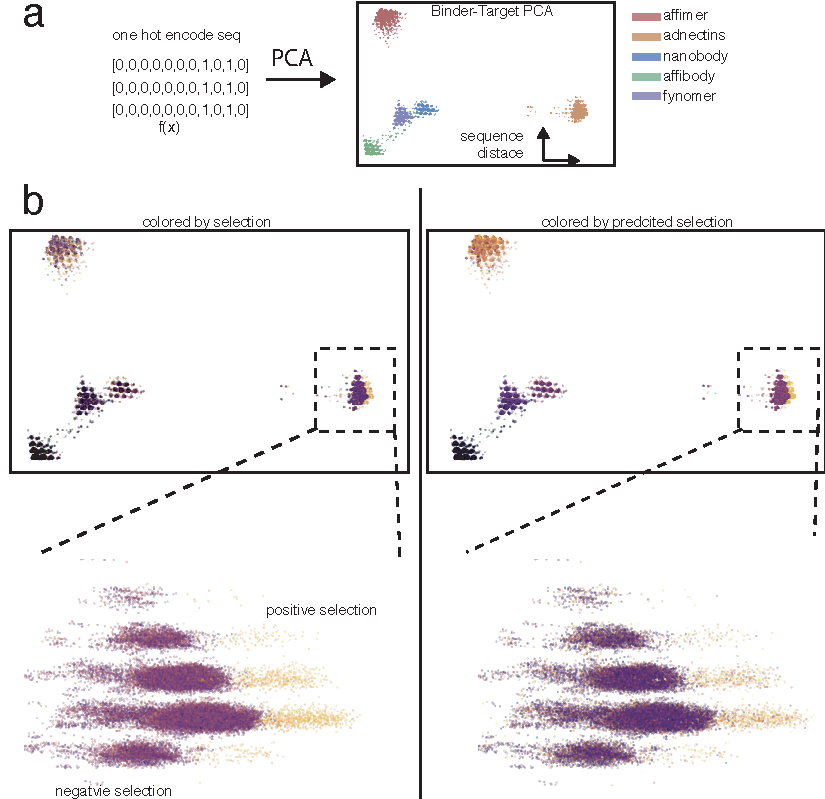
\includegraphics[width=\textwidth]{figures/chapter3/20190621_fig8b_model_pca.pdf}
\caption[Principle components analysis highlights sequence features learned in model]{\textbf{Principle components analysis highlights sequence features learned in model}
\label{chap3-pca}}
\end{figure}
Regression models across all interaction pairs were trained in an effort to approximate information contained within the data. Models trained on only the binder or target sequence performed moderately well within their domain, and poorly across different binding or target domains (Fig\ref{chap3-model}x). Surprisingly, linear models which are trained on global data (all binders, all targets with 25\% data held out for model performance test purposes), are capable of achieving Pearson coefficients of ~.6, showing a strong understanding of the data (Fig\ref{chap3-model}x). Simple single hidden layer neural networks (multi-layer perceptron: mlp)  were capable of achieving Pearson of .7 and mean squared error (MSE) of .004 on held out test data (Fig\ref{chap3-model}b). Global models trained on only the cytokine target class can generalize quite well to the transcription factor activator target class as well, however the inverse is not true (Fig\ref{chap3-model-pca}x). This is likely possibly due to data imbalance (more data in the cytokine class) or diversity structure within the target class. 

% Figure 9: Predictions of binder specificity provide insights into binder phenotypes
\begin{figure}
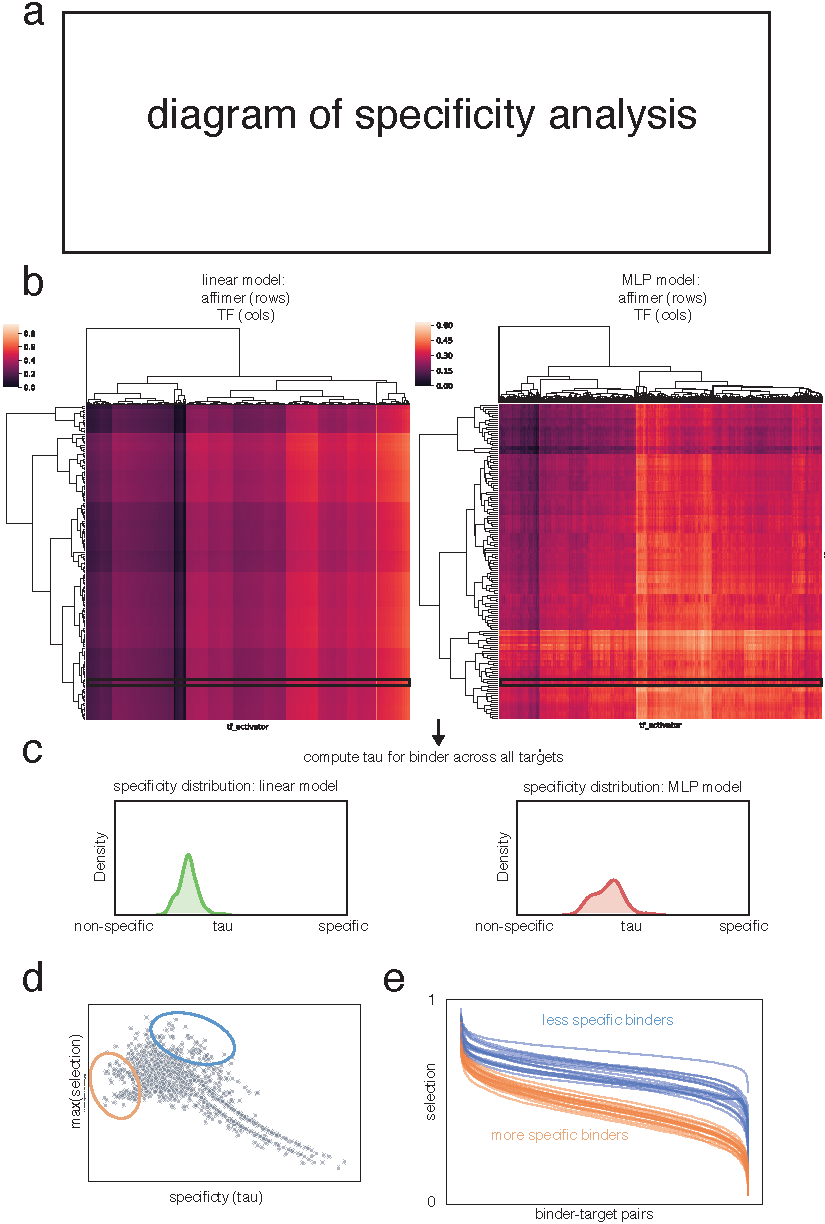
\includegraphics[width=\textwidth]{figures/chapter3/20190622_figure9_specificity.pdf}
\caption[MLP model of interactions learns complex specificity patterns, differentiating binder phenotypes]{\textbf{MLP model of interactions learns complex specificity patterns, differentiating binder phenotypes}
\label{chap3-model-specificty}}
\end{figure}

In an effort to better understand how sequence relates to model reliability, the one hot encoded data for all binder-targets sequences was embedded into a PCA (Fig\ref{chap3-pca}a). The first two components separate the data clearly by binder (Fig\ref{chap3-pca}a). Points were colored by predicted selection from the MLP model as well as the true selection values (Fig\ref{chap3-pca}b). Certain binder regions predictions matched better than others, with the adnectin group showing clear sequence relationships well understood. However the complexity of the data limits how much can be learned from this approach, since there is no “center” sequence we can extrapolate from. 

One of the primary goals of doing a massively multiplexed library on library experiment across many binding modalities and targets is to be able to predict binder specificity. Using predictions of binder specificity could suggest paths to better binders with both high affinity and specificity in the competitive context of the cell.  These models can be used to score binders both seen in the data as well as binders not observed, enabling construction of specificity metrics not currently employed on binders dude to the general lack of required data. For this test, both specific and nonspecific binders were held out from training, and model predictions were tested on these binder sequences across all possible targets contained in the set (whether viewed or not) (Fig\ref{chap3-model-specificty}a). Using these predictions, we calculated a tau score, normally used in gene expression across tissues (cite tau paper) to determine how specific a binder was across all possible targets. Interestly, the linear models gave more “flat” predictions for a binder---usually high or low selection values across large sets of targets---when compared to the mlp models. The MLP model was able to predict the specificity of binding across unseen binders, indicating an ability to generalize information about interactions across diverse arrays of data (Fig\ref{chap3-model-specificty}b). From these predictions, binders can be classed into specific and non-specific, and tested to determine the best possible binders to use in research and therapeutics. This type of model performance can be used to inform subsequent rounds of design of binder target interactions, enabling the next generation of highly specific binders(Fig\ref{chap3-model-specificty}c/d). 

\section{Discussion}

Here we develop methods which enables us to screen millions of binders by millions of targets, which scales linearly with culture volume. We use this method to test many different binding scaffolds by two diverse sets of target libraries. Using this method, we are able to build a diverse dataset profiling thousands of binder target pairs and their specificity. From this data, we traina machine learning regression model which is able to predict with a pearson R values of ~.6 on a random held out test set. Furthermore we probe specificity of specific binders using this model, showing there are indeed predictions for specific binders as well as broad binders. 

The overarching  goal of this project is to be able to design binders to all proteins in the knowable proteome on demand. Measuring and then train machine learning models against large sets of interactions is the first step towards this goal. Future directions will test these designs in a highly parallel system such as this one to see which ones work and which do not, information which we can further use to update the model in and make predictions of increasing quality. This closed loops systems is one of the main advantages over conventional methods, which provide minimal information to enable future more high quality rounds of design. 

Furthermore, validation of the interactions probed in this system across other systems, such as the intracellular mammalian milieu, or the blood, will need to be performed. While it is likely that there will be interactions which are system-specific (and thus don't interact in mammalian etc), this transfer function is also likely learnable. Further machine learning and experimentation methods will enable deciphering of these transfer functions, allowing for the development of binders which work across many contexts. The methods used in this paper are developed with that goal in mind: split T7 is functional in mammalian cell culture systems, thus enabling an easy transfer from the prokaryotic assay to a mammalian verification. 

Finally, within the overarching goal above is the hope to use this method to develop better therapeutic binding proteins. This goal not only requires strong and specific binding, but also other molecular properties which are not addressed in this chapter, such as low immunogenicity. The goal of the methods above is to be able to design many possible binder sequences to a specific target,and it is likely that of these many sequences, some will have different properties in the living body of an organism. This represents a final, unrelated area of missing design and understanding.  Methods which enable testing of thousands of possible protein binders in vivo do not yet exist, but it is likely they will be empowered by the synthesis and sequencing strategies outlined in this chapter. We are in the early stages of measurement-driven protein design, and the future full of exciting possibilities. 